\documentclass[twoside]{book}

% Packages required by doxygen
\usepackage{fixltx2e}
\usepackage{calc}
\usepackage{doxygen}
\usepackage[export]{adjustbox} % also loads graphicx
\usepackage{graphicx}
\usepackage[utf8]{inputenc}
\usepackage{makeidx}
\usepackage{multicol}
\usepackage{multirow}
\PassOptionsToPackage{warn}{textcomp}
\usepackage{textcomp}
\usepackage[nointegrals]{wasysym}
\usepackage[table]{xcolor}

% Font selection
\usepackage[T1]{fontenc}
\usepackage[scaled=.90]{helvet}
\usepackage{courier}
\usepackage{amssymb}
\usepackage{sectsty}
\renewcommand{\familydefault}{\sfdefault}
\allsectionsfont{%
  \fontseries{bc}\selectfont%
  \color{darkgray}%
}
\renewcommand{\DoxyLabelFont}{%
  \fontseries{bc}\selectfont%
  \color{darkgray}%
}
\newcommand{\+}{\discretionary{\mbox{\scriptsize$\hookleftarrow$}}{}{}}

% Page & text layout
\usepackage{geometry}
\geometry{%
  a4paper,%
  top=2.5cm,%
  bottom=2.5cm,%
  left=2.5cm,%
  right=2.5cm%
}
\tolerance=750
\hfuzz=15pt
\hbadness=750
\setlength{\emergencystretch}{15pt}
\setlength{\parindent}{0cm}
\setlength{\parskip}{3ex plus 2ex minus 2ex}
\makeatletter
\renewcommand{\paragraph}{%
  \@startsection{paragraph}{4}{0ex}{-1.0ex}{1.0ex}{%
    \normalfont\normalsize\bfseries\SS@parafont%
  }%
}
\renewcommand{\subparagraph}{%
  \@startsection{subparagraph}{5}{0ex}{-1.0ex}{1.0ex}{%
    \normalfont\normalsize\bfseries\SS@subparafont%
  }%
}
\makeatother

% Headers & footers
\usepackage{fancyhdr}
\pagestyle{fancyplain}
\fancyhead[LE]{\fancyplain{}{\bfseries\thepage}}
\fancyhead[CE]{\fancyplain{}{}}
\fancyhead[RE]{\fancyplain{}{\bfseries\leftmark}}
\fancyhead[LO]{\fancyplain{}{\bfseries\rightmark}}
\fancyhead[CO]{\fancyplain{}{}}
\fancyhead[RO]{\fancyplain{}{\bfseries\thepage}}
\fancyfoot[LE]{\fancyplain{}{}}
\fancyfoot[CE]{\fancyplain{}{}}
\fancyfoot[RE]{\fancyplain{}{\bfseries\scriptsize Generated by Doxygen }}
\fancyfoot[LO]{\fancyplain{}{\bfseries\scriptsize Generated by Doxygen }}
\fancyfoot[CO]{\fancyplain{}{}}
\fancyfoot[RO]{\fancyplain{}{}}
\renewcommand{\footrulewidth}{0.4pt}
\renewcommand{\chaptermark}[1]{%
  \markboth{#1}{}%
}
\renewcommand{\sectionmark}[1]{%
  \markright{\thesection\ #1}%
}

% Indices & bibliography
\usepackage{natbib}
\usepackage[titles]{tocloft}
\setcounter{tocdepth}{3}
\setcounter{secnumdepth}{5}
\makeindex

% Hyperlinks (required, but should be loaded last)
\usepackage{ifpdf}
\ifpdf
  \usepackage[pdftex,pagebackref=true]{hyperref}
\else
  \usepackage[ps2pdf,pagebackref=true]{hyperref}
\fi
\hypersetup{%
  colorlinks=true,%
  linkcolor=blue,%
  citecolor=blue,%
  unicode%
}

% Custom commands
\newcommand{\clearemptydoublepage}{%
  \newpage{\pagestyle{empty}\cleardoublepage}%
}

\usepackage{caption}
\captionsetup{labelsep=space,justification=centering,font={bf},singlelinecheck=off,skip=4pt,position=top}

%===== C O N T E N T S =====

\begin{document}

% Titlepage & ToC
\hypersetup{pageanchor=false,
             bookmarksnumbered=true,
             pdfencoding=unicode
            }
\pagenumbering{alph}
\begin{titlepage}
\vspace*{7cm}
\begin{center}%
{\Large Assignment 3 }\\
\vspace*{1cm}
{\large Generated by Doxygen 1.8.13}\\
\end{center}
\end{titlepage}
\clearemptydoublepage
\pagenumbering{roman}
\tableofcontents
\clearemptydoublepage
\pagenumbering{arabic}
\hypersetup{pageanchor=true}

%--- Begin generated contents ---
\chapter{File Index}
\section{File List}
Here is a list of all documented files with brief descriptions\+:\begin{DoxyCompactList}
\item\contentsline{section}{\hyperlink{prob1_8c}{prob1.\+c} \\*Determine class, Network and Host ID of an I\+Pv4 address }{\pageref{prob1_8c}}{}
\item\contentsline{section}{\hyperlink{prob2__client_8c}{prob2\+\_\+client.\+c} \\*Client side code for U\+DP socket programming }{\pageref{prob2__client_8c}}{}
\item\contentsline{section}{\hyperlink{prob2__server_8c}{prob2\+\_\+server.\+c} \\*Server side code for U\+DP socket programming }{\pageref{prob2__server_8c}}{}
\item\contentsline{section}{\hyperlink{prob3_8tcl}{prob3.\+tcl} }{\pageref{prob3_8tcl}}{}
\item\contentsline{section}{\hyperlink{prob4_8tcl}{prob4.\+tcl} }{\pageref{prob4_8tcl}}{}
\item\contentsline{section}{\hyperlink{prob5_8tcl}{prob5.\+tcl} }{\pageref{prob5_8tcl}}{}
\end{DoxyCompactList}

\chapter{File Documentation}
\hypertarget{prob1_8c}{}\section{prob1.\+c File Reference}
\label{prob1_8c}\index{prob1.\+c@{prob1.\+c}}


Determine class, Network and Host ID of an I\+Pv4 address.  


{\ttfamily \#include $<$stdio.\+h$>$}\newline
{\ttfamily \#include $<$string.\+h$>$}\newline
Include dependency graph for prob1.\+c\+:
\nopagebreak
\begin{figure}[H]
\begin{center}
\leavevmode
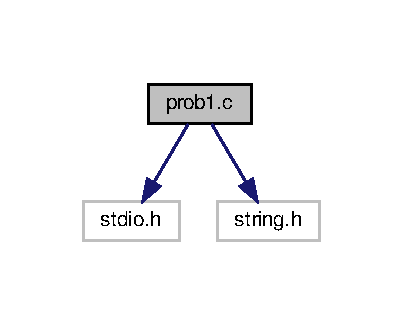
\includegraphics[width=194pt]{prob1_8c__incl}
\end{center}
\end{figure}
\subsection*{Functions}
\begin{DoxyCompactItemize}
\item 
\mbox{\Hypertarget{prob1_8c_a874c2affa0e05eef5dbcd62f0232a591}\label{prob1_8c_a874c2affa0e05eef5dbcd62f0232a591}} 
char {\bfseries find\+Class} (char str\mbox{[}$\,$\mbox{]})
\item 
\mbox{\Hypertarget{prob1_8c_a5f90e3b26836b8a0ff338c925198593d}\label{prob1_8c_a5f90e3b26836b8a0ff338c925198593d}} 
void {\bfseries separate} (char str\mbox{[}$\,$\mbox{]}, char ip\+Class)
\item 
\mbox{\Hypertarget{prob1_8c_ae66f6b31b5ad750f1fe042a706a4e3d4}\label{prob1_8c_ae66f6b31b5ad750f1fe042a706a4e3d4}} 
int {\bfseries main} ()
\end{DoxyCompactItemize}


\subsection{Detailed Description}
Determine class, Network and Host ID of an I\+Pv4 address. 

\begin{DoxyAuthor}{Author}
Ayush Agarwal, 17114017 
\end{DoxyAuthor}
\begin{DoxyDate}{Date}
August 2019 
\end{DoxyDate}

\hypertarget{prob2__client_8c}{}\section{prob2\+\_\+client.\+c File Reference}
\label{prob2__client_8c}\index{prob2\+\_\+client.\+c@{prob2\+\_\+client.\+c}}


Client side code for U\+DP socket programming.  


{\ttfamily \#include $<$arpa/inet.\+h$>$}\newline
{\ttfamily \#include $<$netinet/in.\+h$>$}\newline
{\ttfamily \#include $<$stdio.\+h$>$}\newline
{\ttfamily \#include $<$stdlib.\+h$>$}\newline
{\ttfamily \#include $<$string.\+h$>$}\newline
{\ttfamily \#include $<$sys/socket.\+h$>$}\newline
{\ttfamily \#include $<$sys/types.\+h$>$}\newline
{\ttfamily \#include $<$unistd.\+h$>$}\newline
Include dependency graph for prob2\+\_\+client.\+c\+:
\nopagebreak
\begin{figure}[H]
\begin{center}
\leavevmode
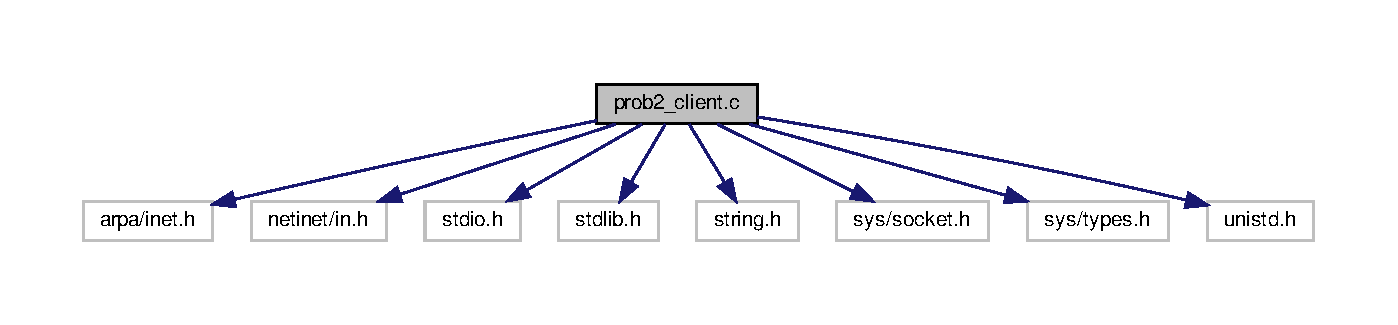
\includegraphics[width=350pt]{prob2__client_8c__incl}
\end{center}
\end{figure}
\subsection*{Macros}
\begin{DoxyCompactItemize}
\item 
\mbox{\Hypertarget{prob2__client_8c_ac0a4ce3bd388c7823743b526e7cb77fb}\label{prob2__client_8c_ac0a4ce3bd388c7823743b526e7cb77fb}} 
\#define {\bfseries I\+P\+\_\+\+P\+R\+O\+T\+O\+C\+OL}~0
\item 
\mbox{\Hypertarget{prob2__client_8c_ad8a262037cbfb38d1512f0073eeb7a66}\label{prob2__client_8c_ad8a262037cbfb38d1512f0073eeb7a66}} 
\#define {\bfseries I\+P\+\_\+\+A\+D\+D\+R\+E\+SS}~\char`\"{}127.\+0.\+0.\+1\char`\"{}
\item 
\mbox{\Hypertarget{prob2__client_8c_a47a4d3bbd05894abbce0ffd1d266aa88}\label{prob2__client_8c_a47a4d3bbd05894abbce0ffd1d266aa88}} 
\#define {\bfseries P\+O\+R\+T\+\_\+\+NO}~15050
\item 
\mbox{\Hypertarget{prob2__client_8c_a30ba2113ad1b0f91029d017fc988d9af}\label{prob2__client_8c_a30ba2113ad1b0f91029d017fc988d9af}} 
\#define {\bfseries N\+E\+T\+\_\+\+B\+U\+F\+\_\+\+S\+I\+ZE}~32
\item 
\mbox{\Hypertarget{prob2__client_8c_abace6f1e028b11cc237bd95c5dbe451a}\label{prob2__client_8c_abace6f1e028b11cc237bd95c5dbe451a}} 
\#define {\bfseries cipher\+Key}~\textquotesingle{}S\textquotesingle{}
\item 
\mbox{\Hypertarget{prob2__client_8c_a6e618c0ec6ffc8ac4489d11c65a5a67c}\label{prob2__client_8c_a6e618c0ec6ffc8ac4489d11c65a5a67c}} 
\#define {\bfseries sendrecvflag}~0
\end{DoxyCompactItemize}
\subsection*{Functions}
\begin{DoxyCompactItemize}
\item 
\mbox{\Hypertarget{prob2__client_8c_a37e9b2e0b0fcbe7d2d5bd9c9467c1fb8}\label{prob2__client_8c_a37e9b2e0b0fcbe7d2d5bd9c9467c1fb8}} 
void {\bfseries clear\+Buf} (char $\ast$b)
\item 
\mbox{\Hypertarget{prob2__client_8c_a4fc6ad5854f646cf1e284f66e104219f}\label{prob2__client_8c_a4fc6ad5854f646cf1e284f66e104219f}} 
char {\bfseries Cipher} (char ch)
\item 
\mbox{\Hypertarget{prob2__client_8c_a0d285ee71db2ee39e24c4a6e552991f3}\label{prob2__client_8c_a0d285ee71db2ee39e24c4a6e552991f3}} 
int {\bfseries recv\+File} (char $\ast$buf, int s)
\item 
\mbox{\Hypertarget{prob2__client_8c_ae66f6b31b5ad750f1fe042a706a4e3d4}\label{prob2__client_8c_ae66f6b31b5ad750f1fe042a706a4e3d4}} 
int {\bfseries main} ()
\end{DoxyCompactItemize}


\subsection{Detailed Description}
Client side code for U\+DP socket programming. 

\begin{DoxyAuthor}{Author}
Ayush Agarwal, 17114017 
\end{DoxyAuthor}
\begin{DoxyDate}{Date}
August 2019 
\end{DoxyDate}

\hypertarget{prob2__server_8c}{}\section{prob2\+\_\+server.\+c File Reference}
\label{prob2__server_8c}\index{prob2\+\_\+server.\+c@{prob2\+\_\+server.\+c}}


Server side code for U\+DP socket programming.  


{\ttfamily \#include $<$arpa/inet.\+h$>$}\newline
{\ttfamily \#include $<$netinet/in.\+h$>$}\newline
{\ttfamily \#include $<$stdio.\+h$>$}\newline
{\ttfamily \#include $<$stdlib.\+h$>$}\newline
{\ttfamily \#include $<$string.\+h$>$}\newline
{\ttfamily \#include $<$sys/socket.\+h$>$}\newline
{\ttfamily \#include $<$sys/types.\+h$>$}\newline
{\ttfamily \#include $<$unistd.\+h$>$}\newline
Include dependency graph for prob2\+\_\+server.\+c\+:
\nopagebreak
\begin{figure}[H]
\begin{center}
\leavevmode
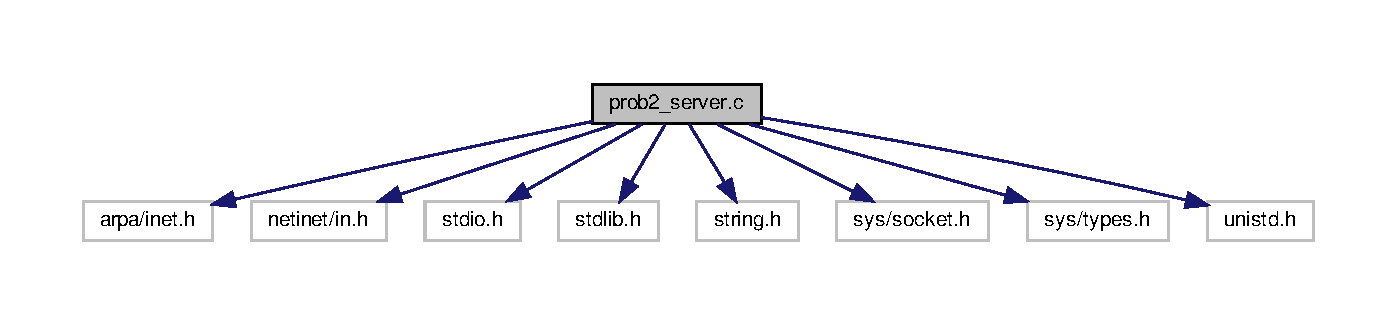
\includegraphics[width=350pt]{prob2__server_8c__incl}
\end{center}
\end{figure}
\subsection*{Macros}
\begin{DoxyCompactItemize}
\item 
\mbox{\Hypertarget{prob2__server_8c_ac0a4ce3bd388c7823743b526e7cb77fb}\label{prob2__server_8c_ac0a4ce3bd388c7823743b526e7cb77fb}} 
\#define {\bfseries I\+P\+\_\+\+P\+R\+O\+T\+O\+C\+OL}~0
\item 
\mbox{\Hypertarget{prob2__server_8c_a47a4d3bbd05894abbce0ffd1d266aa88}\label{prob2__server_8c_a47a4d3bbd05894abbce0ffd1d266aa88}} 
\#define {\bfseries P\+O\+R\+T\+\_\+\+NO}~15050
\item 
\mbox{\Hypertarget{prob2__server_8c_a30ba2113ad1b0f91029d017fc988d9af}\label{prob2__server_8c_a30ba2113ad1b0f91029d017fc988d9af}} 
\#define {\bfseries N\+E\+T\+\_\+\+B\+U\+F\+\_\+\+S\+I\+ZE}~32
\item 
\mbox{\Hypertarget{prob2__server_8c_abace6f1e028b11cc237bd95c5dbe451a}\label{prob2__server_8c_abace6f1e028b11cc237bd95c5dbe451a}} 
\#define {\bfseries cipher\+Key}~\textquotesingle{}S\textquotesingle{}
\item 
\mbox{\Hypertarget{prob2__server_8c_a6e618c0ec6ffc8ac4489d11c65a5a67c}\label{prob2__server_8c_a6e618c0ec6ffc8ac4489d11c65a5a67c}} 
\#define {\bfseries sendrecvflag}~0
\item 
\mbox{\Hypertarget{prob2__server_8c_a49e1fa6b4860231cbcb87bd74f65569f}\label{prob2__server_8c_a49e1fa6b4860231cbcb87bd74f65569f}} 
\#define {\bfseries nofile}~\char`\"{}File Not Found!\char`\"{}
\end{DoxyCompactItemize}
\subsection*{Functions}
\begin{DoxyCompactItemize}
\item 
\mbox{\Hypertarget{prob2__server_8c_a37e9b2e0b0fcbe7d2d5bd9c9467c1fb8}\label{prob2__server_8c_a37e9b2e0b0fcbe7d2d5bd9c9467c1fb8}} 
void {\bfseries clear\+Buf} (char $\ast$b)
\item 
\mbox{\Hypertarget{prob2__server_8c_a4fc6ad5854f646cf1e284f66e104219f}\label{prob2__server_8c_a4fc6ad5854f646cf1e284f66e104219f}} 
char {\bfseries Cipher} (char ch)
\item 
\mbox{\Hypertarget{prob2__server_8c_a19fc2d7afbfbca5d5b78534e8eeb6b29}\label{prob2__server_8c_a19fc2d7afbfbca5d5b78534e8eeb6b29}} 
int {\bfseries send\+File} (F\+I\+LE $\ast$fp, char $\ast$buf, int s)
\item 
\mbox{\Hypertarget{prob2__server_8c_ae66f6b31b5ad750f1fe042a706a4e3d4}\label{prob2__server_8c_ae66f6b31b5ad750f1fe042a706a4e3d4}} 
int {\bfseries main} ()
\end{DoxyCompactItemize}


\subsection{Detailed Description}
Server side code for U\+DP socket programming. 

\begin{DoxyAuthor}{Author}
Ayush Agarwal, 17114017 
\end{DoxyAuthor}
\begin{DoxyDate}{Date}
August 2019 
\end{DoxyDate}

\hypertarget{prob3_8tcl}{}\section{prob3.\+tcl File Reference}
\label{prob3_8tcl}\index{prob3.\+tcl@{prob3.\+tcl}}
\subsection*{Functions}
\begin{DoxyCompactItemize}
\item 
\mbox{\Hypertarget{prob3_8tcl_a30728837c246b65ef76298af0101d99c}\label{prob3_8tcl_a30728837c246b65ef76298af0101d99c}} 
{\bfseries finish}
\end{DoxyCompactItemize}


\subsection{Detailed Description}
Aim -\/ To monitor traffic for Star topology using N\+S2 \begin{DoxyVerb}
\end{DoxyVerb}

\hypertarget{prob4_8tcl}{}\section{prob4.\+tcl File Reference}
\label{prob4_8tcl}\index{prob4.\+tcl@{prob4.\+tcl}}
\subsection*{Functions}
\begin{DoxyCompactItemize}
\item 
\mbox{\Hypertarget{prob4_8tcl_a30728837c246b65ef76298af0101d99c}\label{prob4_8tcl_a30728837c246b65ef76298af0101d99c}} 
{\bfseries finish}
\end{DoxyCompactItemize}


\subsection{Detailed Description}
Aim -\/ To monitor traffic for Ring topology using N\+S2

\begin{DoxyVerb}
\end{DoxyVerb}

\hypertarget{prob5_8tcl}{}\section{prob5.\+tcl File Reference}
\label{prob5_8tcl}\index{prob5.\+tcl@{prob5.\+tcl}}
\subsection*{Functions}
\begin{DoxyCompactItemize}
\item 
\mbox{\Hypertarget{prob5_8tcl_a30728837c246b65ef76298af0101d99c}\label{prob5_8tcl_a30728837c246b65ef76298af0101d99c}} 
{\bfseries finish}
\end{DoxyCompactItemize}


\subsection{Detailed Description}
Aim -\/ To monitor traffic for Bus topology using N\+S2

\begin{DoxyVerb}
\end{DoxyVerb}

%--- End generated contents ---

% Index
\backmatter
\newpage
\phantomsection
\clearemptydoublepage
\addcontentsline{toc}{chapter}{Index}
\printindex

\end{document}
